\newpage
\section{The Method of Least Squares}
\nl\textbf{A.) The probabalistic construction:}

\nl Given all possible lines $y=mx+b$ that \textit{could} describe the data, the \say{most likely} one will be a line that intersects the point $(\mu_x, \mu_y)$.

\nl That is $y - \mu_y = m(x-\mu_x)$. Because we are interpreting $y$ and a function of $x$, the \say{best line} should be one that minimizes the vertical distance (error (residuals)) in the $y$-direction.

\nl For a point $(x_k,\, y_k)$ in $S$, the vertical distaince is 
$$\text{dist} = \abs{y_k - \big(m(x_k - \mu_x) + \mu_y \big)}.$$
Minimizing absolute values is a pain, but calculus I suggests we square this,
$$\operatorname{dist}^2 = \Big((y_k-\mu_y) - m(x_k-\mu_x)\Big)^2.$$
As $x,y$ are distributed via some PDF, the best way to compute our minimization problem is to minimize expectation with respect to slope $m$:
$$K(m) := \E{\operatorname{dist}^2(m)} = \underbrace{\E{\Big((y_k-\mu_y) - m(x_k-\mu_x)\Big)^2}}_{\setRed **}.$$
\setRed ** \setBlack The $m$ that minimizes is called the solution to our \underline{least-squares problem}.
\begin{align*}
    K(m) &= \E{(y_k-\mu_y)^2  -2m(x_k-\mu_x)(y_k - \mu_y) + m^2(x_k-\mu_x)^2 }\\
    &= \E{(y_k-\mu_y)^2} -2m \E{(x_k-\mu_x)(y_k - \mu_y) } + m^2\E{(x_k-\mu_x)^2}\\
    &= S^2_y - 2m \Cov(X,Y) + m^2S^2_x
\end{align*}
Minimizing (with respect to $m$) $\dfrac{\partial}{\partial m}$,
$$K'(m) = -2 \Cov(X,Y) - 2mS^2_x.$$
With $K'(m) = 0$ then $m = \dfrac{\Cov(X,Y)}{S^2_x}$. 

\nl Note that by the second derivitive test, $K''(m) = 2S_x^2 > 0$. In AP Stats (MTH 111), the slope is moved to a \say{prettier} form:

\begin{align*}
    m &= \frac{\Cov(X,Y)}{S_x^2} \\
    &= \frac{\Cov(X,Y)}{S_x S_y} \cdot \frac{S_y}{S_x}\\
    &= \rho \cdot \frac{S_y}{S_x} \hspace{1in} \rho := \frac{\Cov(X,Y)}{S_xS_y}
\end{align*}

\nl \bu{FACT \#1}: The sign of the slope depends entirely upon $\rho$, where the sign is dependent upon $\Cov(X,Y)$

\nnl \bu{FACT \#2}: $-1 \leq \rho \leq 1$.

\nl (For my MTH 325 class, we proved this fact in full generality).

\nnl \bu{FACT \#3}: The closer $\abs{\rho}$ is to 1, the better the line $\widehat{y} = mx+b$ \say{fits} the data.
\begin{center}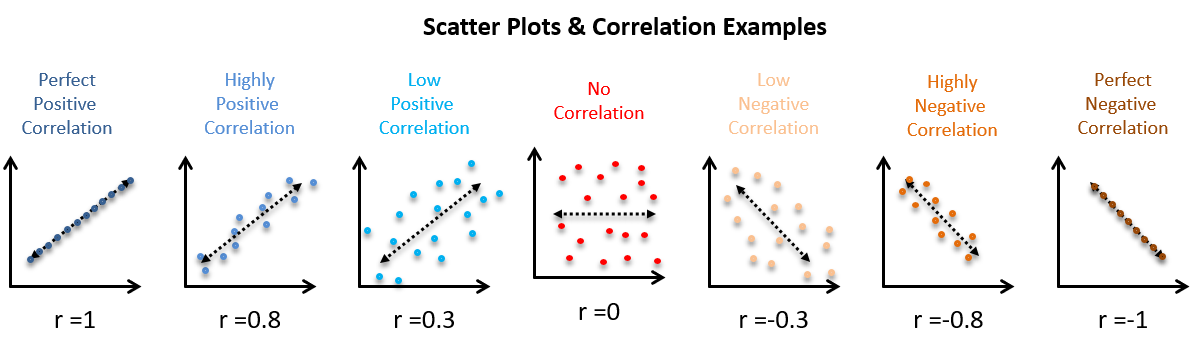
\includegraphics[width=6in]{ch11_scatter.png}\end{center}

\nl The AP Stats definition fo the best fit line is $\widehat{y} = \widehat{b}_0 + \widehat{b}_1x$ where $\widehat{b}_1 = \rho \dfrac{S_y}{S_x}$ and $\widehat{b}_0 = \bar{y} - \widehat{b}_1 \bar{x}$.

\nnl\textbf{B.) The linear algebra construction:}

\nl We still have $S = \{(x_k,\, y_k)\}$. We want $y = mx+b$. Using $S$ always yields an overdetermined (i.e. inconsistent) system
\begin{align*}
    y_1 &= mx_1 + b\\
    y_2 &= mx_2 + b\\
    & \;\;\vdots\\
    y_n &= mx_n + b.
\end{align*}
This is $n$ equations with 2 variables, but we can rewrite as vector equations. $$\vec{y} = m\vec{x} + b \vec{1} \quad \text{where } \vec{y} = \thru{y}, \vec{x} = \thru{x}, \text{ and } \vec{1} = \underbrace{(1,1,\dots,1)}_{n \text{ components}}.$$

\nl Trying to write $\vec{y}$ as a linear combination of $\vec{x}$ and $\vec{1}$. Consider the plane $P = \operatorname{span}\{\vec{x},\vec{1}\}$. Inconsistent implies that $\vec{y} \not \in P$.

\nl But the vector in $P$ that is closest to $\vec{y}$ is $\operatorname{proj}_P\vec{y}$. (Closest under Euclidean distance), recall $\inner{u,v} = u \cdot v$ in $\R^n$.
$$\operatorname{dist}^2 = \sum (y_i - v_i)^2, \quad \vec{v} \in P = \underbrace{\vec{y} \cdot \vec{v} = \inner{y,v}}_{\substack{\text{\say{least squares}}}}$$
\begin{center}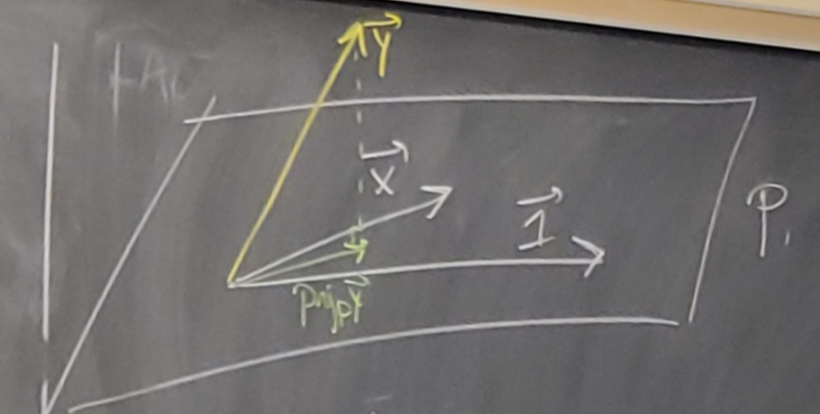
\includegraphics[width=4in]{ch11_proj.png}\end{center}

\noindent Easiest way to project onto $P$ is to have an orthogonal basis for $P$. We need an orthogonal basis for $P$: 
\begin{center}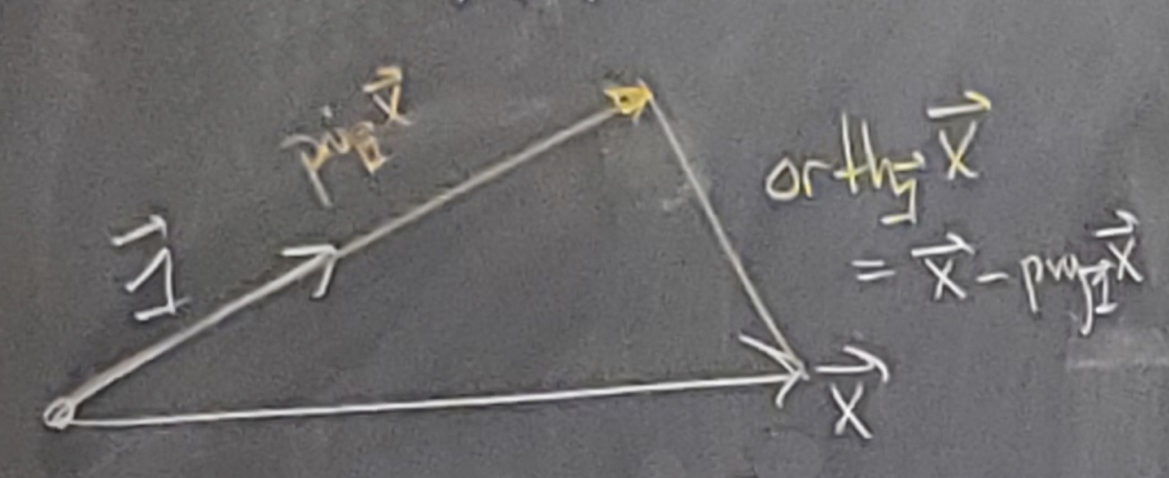
\includegraphics[width=4in]{ch11_basis.png}\end{center}

\nl $P = \operatorname{span}\left\{1, \, \operatorname{orth}_{1}x \right\} = \operatorname{span}\left\{1,\, v\right\}$ where
\begin{align*}
    v &= x - \proj{1}{x}\\
    &= x - \frac{\inner{x,1}}{\inner{1,1}}{1}\\
    &= x - \frac{\inner{x,1}}{n}{1}
\end{align*}
Then 
\begin{align*}
    \proj{P}{y} &= \frac{\inner{y,1}}{\inner{1,1}}1 + \frac{\inner{y,v}}{\inner{v,v}} v\\
    &= \frac{\inner{y,1}}{n}{1} + \frac{\inner{y,v}}{\inner{v,v}}x -\frac{\inner{y,v}}{\inner{v,v}} \cdot \frac{\inner{x,1}}{n}{1}\\
    &= \underbrace{\frac{\inner{y,v}}{\inner{v,v}}}_{\setGreen\substack{\textstyle m\\  \textstyle\text{(slope)}}}x + \underbrace{\pars{\frac{\inner{y,1}}{n} - \frac{\inner{y,v}}{\inner{v,v}}\cdot\frac{\inner{x,1}}{n}}}_{ \setGreen \substack{\textstyle b\\\textstyle\text{(}y \text{-intercept)}}}1
\end{align*}

\begin{align*}
    \inner{v,v} &= \inner{x - \frac{\inner{x,1}}{n}1,\; x - \frac{\inner{x,1}}{n}1}\\
    &= \inner{x,x} -2 \inner{x,\; \frac{\inner{x,1}}{n}1} + \inner{\frac{\inner{x,1}}{n}1,\; \frac{\inner{x,1}}{n}1}\\
    &= \inner{x,x} - 2 \frac{\inner{x,1}}{n}\inner{x,1} + \frac{\inner{x,1}^2}{n^2}\inner{1,1}\\
    &= \inner{x,x} - 2 \frac{\inner{x,1}^2}{n} + \frac{\inner{x,1}^2}{n}\\
    &= \frac{n \inner{x,x} - \inner{x,1}^2}{n}
    %
    %&= \inner{x,x} - 2 \frac{\inner{x,1}^2}{n} + \inner{\frac{\inner{x,1}^2}{n^2}1 ,\; 1}\\
    %&= x \cdot x - 2 \frac{\inner{x,1}^2}{n} + \frac{\inner{x,1}^2}{n}\\
    %&= \frac{n\inner{x,n} - \inner{x,1}^2}{n}
\end{align*}

\begin{align*}
    \inner{v,y} &= \inner{x,y} - \frac{\inner{x,1}\inner{y,1}}{n}\\
    &= n\inner{x,y} - \inner{x,1}\inner{y,1}
\end{align*}
Then
\begin{align*}
    m &= \frac{\inner{v,y}}{\inner{v,v}}\\
    &= \setBlue\frac{n\inner{x,y} - \inner{x,1}\inner{y,1}}{n\inner{x,x} - \inner{x,1}^2}
\end{align*}

% ^^^^ monday to finish

\noindent Then % b = (y dot 1 / n)    -    m (x dot 1 / n)
\begin{align*}
    b &= \frac{\inner{y,1}}{n} - m \frac{\inner{x,1}}{n}\\
    &= \bar{y} - m \bar{x}
\end{align*}
Which is what we got form the probabalistic approach.

\nnl Claim: The two-sets of formulas are identical

\begin{align*}
    m &= \frac{\Cov(X,Y)}{S_x^2} = \rho \frac{S_y}{S_x}\\
    &= \frac{\sum(x_i-\bar{x})(y_i-\bar{y})}{\sum (x_i - \bar{x})^2}
\end{align*}
Useful formula:
\begin{align*}
    \sum (x_i - \bar{x})(y_i - \bar{y}) &= \sum (x_i y_i - x_i \bar{y} - y_i \bar{x} + \bar{x}\bar{y})\\
    &= \sum x_i y_i - \bar{y} \sum x_i - \bar{x} y_i + \bar{x}\bar{y} \sum 1\\
    &= \sum x_i y_i - \bar{y} n \cdot \over{n} \sum x_i - \bar{x} n \cdot \over{n} \sum y_i + n \bar{x} \bar{y}\\
    &= \sum x_iy_i - n \bar{x} \bar{y} -  n\bar{x} \bar{y} +  n\bar{x} \bar{y}\\
    &= \sum x_i y_i - n\bar{x} \bar{y}
\end{align*}

\begin{align*}
    m &= \frac{\Cov(X,Y)}{S_x^2} = \rho \frac{S_y}{S_x}\\
    &= \frac{\sum(x_i-\bar{x})(y_i-\bar{y})}{\sum (x_i - \bar{x})^2}\\
    &= \frac{\sum x_iy_i - n  \bar{x} \bar{y}}{\sum x_i^2 - n \bar{x}^2}\\
    &= \frac{\inner{x,y} - n \pfrac*{\inner{x,1}}{n} \pfrac*{\inner{y,1}}{n} }{\inner{x,x} - n \pfrac*{\inner{x,1}}{n}^2}\\
    &= \setBlue \frac{n\inner{x,y} - \inner{x,1}\inner{y,1}}{n \inner{x,x} - \inner{x,1}^2}\\
    &= \frac{n\sum x_i y_i - \pars{\sum x_i}\pars{\sum y_i}}{n \sum x_i^2 - \pars{\sum x_i}^2}\\
    &= m
\end{align*}

